\section{Identification}\label{sec:identification}

As outlined in \cref{sec:techniques} above, a key challenge is identifying and isolating the various components which are going to be analysed. \cref{sec:segmentation} outlines from the research conducted and which methods were selected for segmentation, feature extraction and allocation of pitch, duration and other properties.

\subsection{Segmentation}\label{sec:segmentation}

In order to perform a decomposition of the manuscript, within \noteED I perform multiple stages of segmentation combined with classification. For the purposes of demonstration I will be following the identification process using the manuscript example in \cref{fig:canvas-initial}.

\begin{figure}[hbt]
  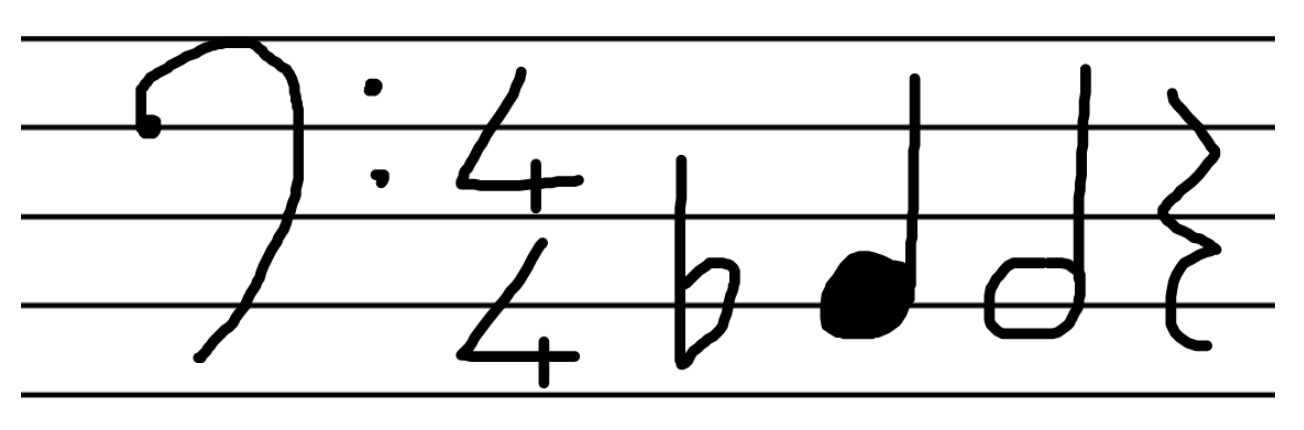
\includegraphics[width=\linewidth]{gfx/techniques/labelling/initial.png}
  \caption{The initial clean manuscript attempt}
  \label{fig:canvas-initial}
\end{figure}
\subsubsection{Initial Segmentation}

Connected component analysis (see \cref{sec:connected-component-analysis}) is performed to isolate the individual components on the stave, resulting in the first stage of component segmentation seen in \cref{fig:canvas-segmentation-1}.

\begin{figure}[hbt]
  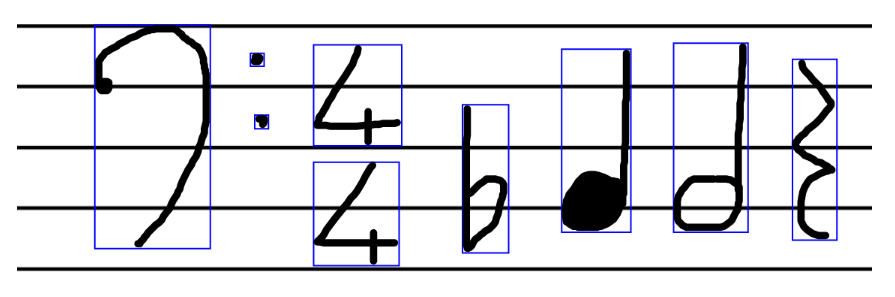
\includegraphics[width=\linewidth]{gfx/techniques/labelling/initial-segmentation.png}
  \caption{After initial segmentation of \cref{fig:canvas-initial}}
  \label{fig:canvas-segmentation-1}
\end{figure}

The components are then classified using the first of two KNN classifiers (KNN1 - discussed below in \cref{sec:implementation-classification}) which results in the basic labelling of the manuscript components seen in \cref{fig:canvas-classified-1}.

\begin{figure}[hbt]
  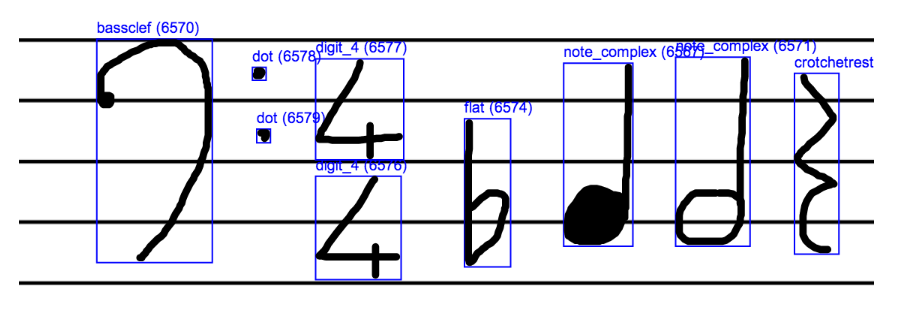
\includegraphics[width=\linewidth]{gfx/techniques/labelling/initial-classification.png}
  \caption{After first level classification of \cref{fig:canvas-segmentation-1}}
  \label{fig:canvas-classified-1}
\end{figure}

The \emph{note\_complex} and \emph{split\_x/split\_y} components are divided into sub-components using techniques such as stem removal (\cref{sec:stem-removal}) and vertical projections (\cref{sec:projections}) respectively. The new set of components are classified using one of the specialised classifiers, the original KNN1 classifier in the case of split components or the KNN2 classifier for note subcomponents to produce the more detailed component labelling in \cref{fig:canvas-segmentation-classification-2}.

\begin{figure}[hbt]
  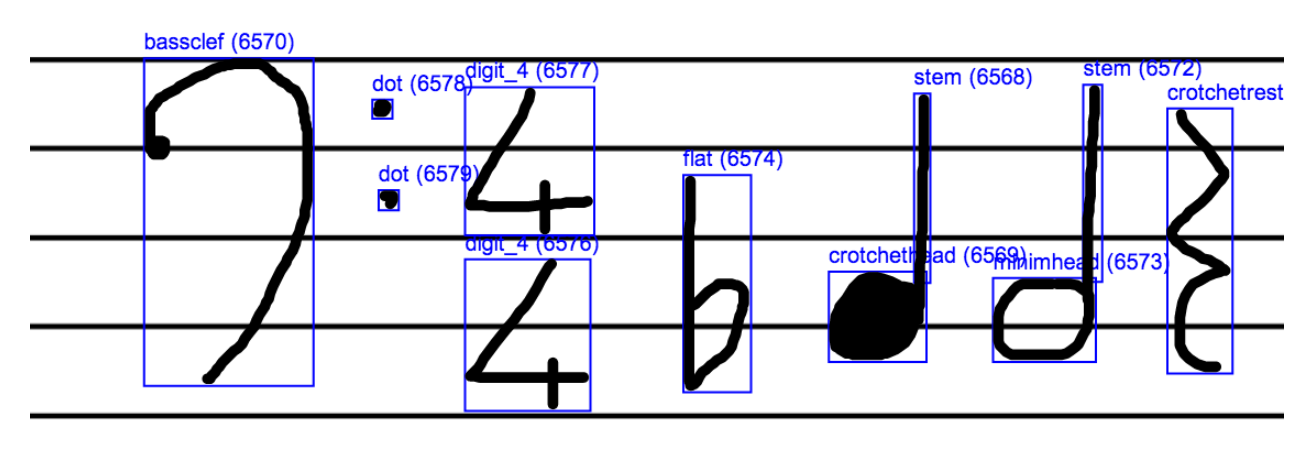
\includegraphics[width=\linewidth]{gfx/techniques/labelling/secondary-segmentation-classification.png}
  \caption{After second level segmentation and classification of \cref{fig:canvas-classified-1}. Note the stems are now labelled}
  \label{fig:canvas-segmentation-classification-2}
\end{figure}

No further segmentation is performed on the components after this point.

\subsubsection{Stem Removal}\label{sec:stem-removal}

In order to split up a \emph{note\_complex} into heads, tails, beam, stem etc, the first step is to try and isolate the stems. We can do this by removing horizontal runs of black pixels which are above a threshold greater than the typical width of a stem. Since runs like this appear at the intersection of the stem with other components, the result is a large number of new regions in the image, one of which is likely to be the stem.

To establish which region is a stem and remove any noise, we look for regions which are within a set aspect ratio (I use $1:2$, obtained experimentally and designed to catch angled stems as well as very vertical ones) and a height above a minimum threshold (I use $40$px, also obtained experimentally).

\begin{figure}[H]
  \centering

  \begin{subfigure}[b]{.2\linewidth}
      \centering
      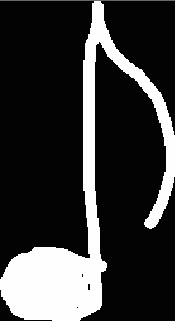
\includegraphics[width=\linewidth]{gfx/techniques/stem-detection-1.png}
      \caption{The original component}
      \label{fig:stem-segmentation-1}
  \end{subfigure}
  \begin{subfigure}[b]{.2\linewidth}
      \centering
      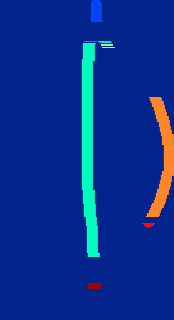
\includegraphics[width=\linewidth]{gfx/techniques/stem-detection-2.png}
      \caption{The original component}
      \label{fig:stem-segmentation-2}
  \end{subfigure}
  \begin{subfigure}[b]{.2\linewidth}
      \centering
      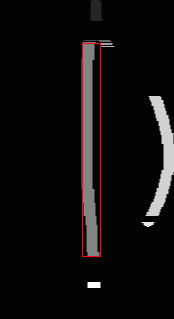
\includegraphics[width=\linewidth]{gfx/techniques/stem-detection-3.png}
      \caption{The original component}
      \label{fig:stem-segmentation-3}
  \end{subfigure}
  \begin{subfigure}[b]{.2\linewidth}
      \centering
      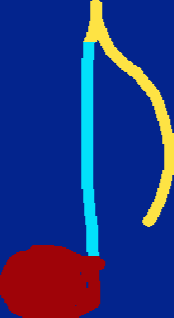
\includegraphics[width=\linewidth]{gfx/techniques/stem-detection-4.png}
      \caption{The original component}
      \label{fig:stem-segmentation-4}
  \end{subfigure}

  \caption{The stages in stem detection for sharps}
  \label{fig:bar-line-types}
\end{figure}


\subsection{Feature Extraction}

\subsubsection{Resampling}

Using the pixels of an image as the features is an approach used in several of the papers I looked at \todo{Reference papers using images + resampling over features}, however in order to be able to compare feature vectors, they need to be the same size which means we need to resize the images to a common dimension.

To do this, I resize the images down using bilinear interpolation to an experimentally obtained dimension of $20\times50$px obtained in \cref{sec:knn}. The smaller dataset increases the speed at which a classifier can operate and I also found it to be comparable to if not more accurate than the feature vectors of larger images (\cref{table:knn-width-height-top}).

\subsubsection{Statistical Properties}
\label{sec:statistical-properties}

For my experimental statistical feature vector, I use techniques outlined in \cref{sec:component-features} to generate a feature vector comprising of the following properties:

\todo[inline,color=red]{Statistical Properties List which didn't bloody work}

\subsection{Classification}
\label{sec:implementation-classification}

Classifiers are created by taking a sets of previously labelled samples and building a model which provides the most accurate relation between the samples and their labels. This allows new samples to be classified using the model to apply the most likely (and hopefully, correct) label.

In order to maximise the accuracy of my classifications, I ran multiple experiments on different classifiers before deciding on which one I would apply in my application.

\subsubsection{K Nearest Neighbour}\label{sec:knn}

For the K Nearest Neighbour algorithm, I tried two different feature vectors, the first was using the statistical properties outlined in \cref{sec:statistical-properties} and the second was a resampled binary image flattened into a 1D array.

\paragraph{Statistical Feature Vector}
\label{sec:knn-stats}

An initial attempt at classification using statistical properties and a KNN classifier wasn't all that successful as you can see from the confusion matrix and accuracy scores in \cref{fig:knn-stats}. Most components were incorrectly classified as crotchet heads though I was unable to come up with a good explanation as to why and it's something which it would be interesting to investigate further in future.

\begin{table}
  \centering
  \begin{subtable}[b]{\linewidth}
    \tiny
    \begin{tabularx}{\textwidth}{r|XXXXXXXXXXXXXXXXXXXXXX}
         & \rot{crotchetrest}  & \rot{minimhead}  & \rot{note\_complex}  & \rot{bassclef}  & \rot{beam\_complex}  & \rot{sharp}  & \rot{semibreve}  & \rot{quaverrest}  & \rot{barline}  & \rot{quavertaildown}  & \rot{minimsemibreverest}  & \rot{flat}  & \rot{crotchethead}  & \rot{stem}  & \rot{trebleclef}  & \rot{digit\_8}  & \rot{natural}  & \rot{digit\_3}  & \rot{digit\_2}  & \rot{digit\_4}  & \rot{quavertailup}  & \rot{dot} \\
      \midrule
    crotchetrest & 0 & 0 & 0 & 0 & 0 & 0 & 0 & 0 & 0 & 0 & 0 & 0 & 44 & 0 & 0 & 0 & 0 & 0 & 0 & 0 & 0 & 0 \\
    minimhead & 0 & 16 & 0 & 0 & 0 & 0 & 0 & 0 & 0 & 0 & 0 & 0 & 48 & 0 & 0 & 0 & 0 & 0 & 0 & 0 & 0 & 0 \\
    note\_complex & 0 & 0 & 32 & 0 & 0 & 0 & 0 & 0 & 0 & 0 & 0 & 0 & 87 & 0 & 0 & 0 & 0 & 0 & 0 & 0 & 0 & 0 \\
    bassclef & 0 & 0 & 0 & 0 & 0 & 0 & 0 & 0 & 0 & 0 & 0 & 0 & 37 & 0 & 0 & 0 & 0 & 0 & 0 & 0 & 0 & 0 \\
    beam\_complex & 0 & 0 & 0 & 0 & 0 & 0 & 0 & 0 & 0 & 0 & 0 & 0 & 1 & 0 & 0 & 0 & 0 & 0 & 0 & 0 & 0 & 0 \\
    sharp & 0 & 0 & 0 & 0 & 0 & 6 & 0 & 0 & 0 & 0 & 0 & 0 & 46 & 0 & 0 & 0 & 0 & 0 & 0 & 0 & 0 & 0 \\
    semibreve & 0 & 0 & 0 & 0 & 0 & 0 & 1 & 0 & 0 & 0 & 0 & 0 & 37 & 0 & 0 & 0 & 0 & 0 & 0 & 0 & 0 & 0 \\
    quaverrest & 0 & 0 & 0 & 0 & 0 & 0 & 0 & 0 & 0 & 0 & 0 & 0 & 36 & 0 & 0 & 0 & 0 & 0 & 0 & 0 & 0 & 0 \\
    barline & 0 & 0 & 0 & 0 & 0 & 0 & 0 & 0 & 0 & 0 & 0 & 0 & 32 & 0 & 0 & 0 & 0 & 0 & 0 & 0 & 0 & 0 \\
    quavertaildown & 0 & 0 & 0 & 0 & 0 & 0 & 0 & 0 & 0 & 0 & 0 & 0 & 10 & 0 & 0 & 0 & 0 & 0 & 0 & 0 & 0 & 0 \\
    minimsemibreverest & 0 & 0 & 0 & 0 & 0 & 0 & 0 & 0 & 0 & 0 & 1 & 0 & 9 & 0 & 0 & 0 & 0 & 0 & 0 & 0 & 0 & 0 \\
    flat & 0 & 0 & 0 & 0 & 0 & 0 & 0 & 0 & 0 & 0 & 0 & 2 & 50 & 0 & 0 & 0 & 0 & 0 & 0 & 0 & 0 & 0 \\
    crotchethead & 0 & 0 & 0 & 0 & 0 & 0 & 0 & 0 & 0 & 0 & 0 & 0 & 133 & 0 & 0 & 0 & 0 & 0 & 0 & 0 & 0 & 0 \\
    stem & 0 & 0 & 0 & 0 & 0 & 0 & 0 & 0 & 0 & 0 & 0 & 0 & 60 & 24 & 0 & 0 & 0 & 0 & 0 & 0 & 0 & 0 \\
    trebleclef & 0 & 0 & 0 & 0 & 0 & 0 & 0 & 0 & 0 & 0 & 0 & 0 & 40 & 0 & 2 & 0 & 0 & 0 & 0 & 0 & 0 & 0 \\
    digit\_8 & 0 & 0 & 0 & 0 & 0 & 0 & 0 & 0 & 0 & 0 & 0 & 0 & 0 & 0 & 0 & 1 & 0 & 0 & 0 & 0 & 0 & 0 \\
    natural & 0 & 0 & 0 & 0 & 0 & 0 & 0 & 0 & 0 & 0 & 0 & 0 & 37 & 0 & 0 & 0 & 0 & 0 & 0 & 0 & 0 & 0 \\
    digit\_3 & 0 & 0 & 0 & 0 & 0 & 0 & 0 & 0 & 0 & 0 & 0 & 0 & 7 & 0 & 0 & 0 & 0 & 2 & 0 & 0 & 0 & 0 \\
    digit\_2 & 0 & 0 & 0 & 0 & 0 & 0 & 0 & 0 & 0 & 0 & 0 & 0 & 9 & 0 & 0 & 0 & 0 & 0 & 0 & 0 & 0 & 0 \\
    digit\_4 & 0 & 0 & 0 & 0 & 0 & 0 & 0 & 0 & 0 & 0 & 0 & 0 & 19 & 0 & 0 & 0 & 0 & 0 & 0 & 7 & 0 & 0 \\
    quavertailup & 0 & 0 & 0 & 0 & 0 & 0 & 0 & 0 & 0 & 0 & 0 & 0 & 11 & 0 & 0 & 0 & 0 & 0 & 0 & 0 & 3 & 0 \\
    dot & 0 & 0 & 0 & 0 & 0 & 0 & 0 & 0 & 0 & 0 & 0 & 0 & 27 & 0 & 0 & 0 & 0 & 0 & 0 & 0 & 0 & 15 \\
    \end{tabularx}
  \end{subtable}

  \vspace{0.8cm}

  \begin{subtable}[b]{.4\linewidth}
    \begin{tabularx}{\linewidth}{lll}
      \toprule
      Accuracy & Precision & Recall \\
      \midrule
      0.275 & 0.645 & 0.275 \\
      \bottomrule
    \end{tabularx}
  \end{subtable}

  \caption{KNN classifier results using statistical features}
  \label{fig:knn-stats}
\end{table}

\paragraph{Image Feature Vector}
\label{sec:knn-image}
For the resampled image features, I ran a series of trials for different dimensions from 10px to 100px in both width and height (in 10px increments), averaging 3 repeats per dimension (each with a different training/testing split) and then generating a matrix of accuracies (which can be seen in full in \cref{table:height-width-matrix}).

Since most objects on a stave have a more vertical aspect ratio, I first graphed the average and maximum of the scores for each different height across all widths to see if there were any trends such as taller images producing higher accuracy.

The results can be seen in \cref{fig:height-resample} and it seemed that in general, very short images ($\leq 20\text{px}$) gave worse results than tall ones but there wasn't anything conclusive and the gains from very tall images as opposed to fairly small images were minimal. Since there wasn't a height which clearly stood out, an analysis of the full matrix was done to find the highest scoring height and width combinations.

The top ten experimental accuracies from the tested dimensions are listed in \cref{table:knn-width-height-top} and I eventually selected $20\times50\text{px}$ as my resampled dimension, the reason being that although larger dimensions did technically produce better accuracies, they were only \emph{slightly} better and would have resulted in many more pixels in the feature vector, slowing down the process of building a classifier and testing samples.

\begin{figure}[H]
  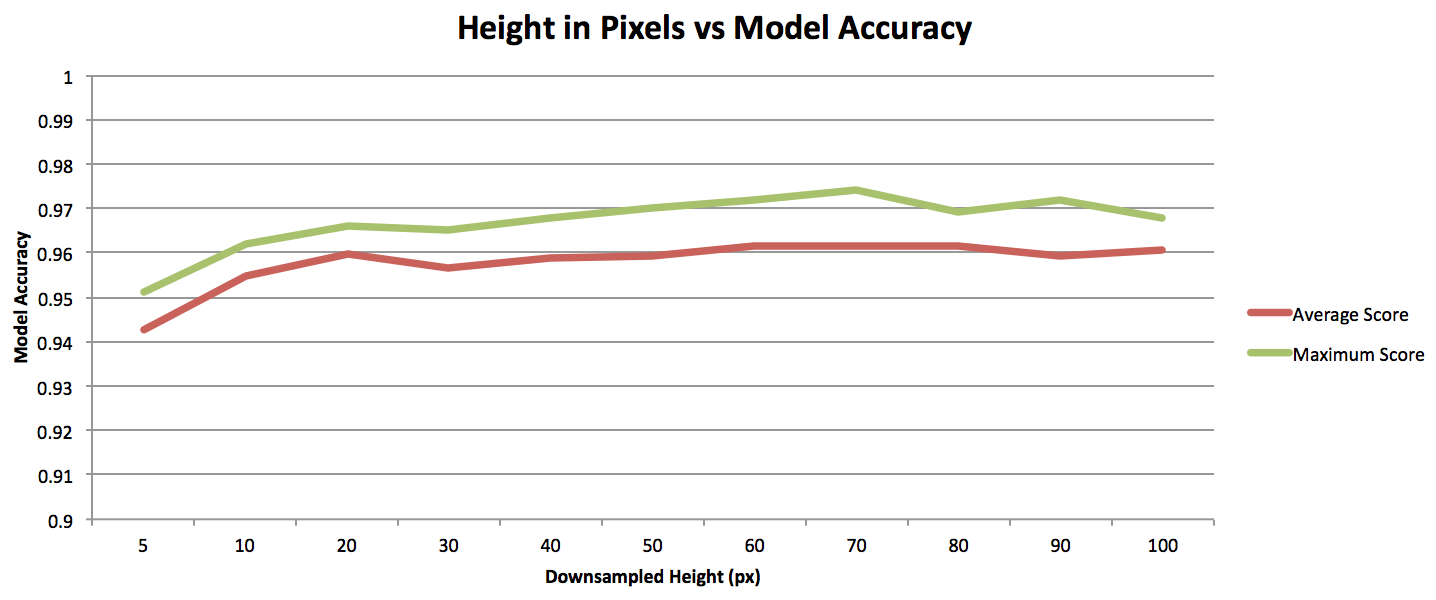
\includegraphics[width=\linewidth]{gfx/techniques/downsampling-height-vs-accuracy.png}
  \caption{The effect of resampled image height on accuracy}
  \label{fig:height-resample}
\end{figure}

\begin{table}[H]

    \begin{tabularx}{\textwidth}{ r X X X X }
    \toprule
    & Width & Height & Total Pixels & Accuracy \\
    \midrule
    & 50  & 70  & 3500 & 0.974 \\
    & 20  & 60  & 1200 & 0.971 \\
    & 20  & 70  & 1400 & 0.97 \\
    $\rightarrow$ & \textbf{20}  & \textbf{50}  & \textbf{1000} & \textbf{0.969} \\
    & 30  & 70  & 2100 & 0.969 \\
    & 100 & 70  & 7000 & 0.969 \\
    & 20  & 40  & 800  & 0.968 \\
    & 70  & 50  & 3500 & 0.967 \\
    & 60  & 60  & 3600 & 0.967 \\
    & 20  & 100 & 2000 & 0.967 \\
    \bottomrule
    \end{tabularx}

    \caption{Top 10 accuracy scores for different width and height combinations, the selection dimensions used in the classifier are highlighted and the full matrix can be found in \cref{table:height-width-matrix}}
    \label{table:knn-width-height-top}
\end{table}

\begin{table}[H]

    \begin{tabularx}{\textwidth}{ lXXXXXXXXXX }
    \toprule
    & \multicolumn{10}{c}{Width (px)} \\
    \cmidrule{2-11}
    Height (px) & 10   & 20   & 30   & 40   & 50   & 60   & 70   & 80   & 90   & 100  \\
    \midrule
    10          & 0.948 & 0.961 & 0.955 & 0.954 & 0.962 & 0.953 & 0.951 & 0.953 & 0.955 & 0.957 \\
    20          & 0.947 & 0.963 & 0.963 & 0.962 & 0.964 & 0.962 & 0.956 & 0.961 & 0.960 & 0.966 \\
    30          & 0.945 & 0.960 & 0.954 & 0.965 & 0.958 & 0.958 & 0.956 & 0.958 & 0.959 & 0.959 \\
    40          & 0.946 & 0.968 & 0.957 & 0.963 & 0.958 & 0.950 & 0.961 & 0.964 & 0.960 & 0.966 \\
    50          & 0.935 & 0.969 & 0.965 & 0.957 & 0.961 & 0.957 & 0.967 & 0.959 & 0.948 & 0.962 \\
    60          & 0.953 & 0.971 & 0.960 & 0.963 & 0.962 & 0.967 & 0.948 & 0.957 & 0.957 & 0.963 \\
    70          & 0.954 & 0.970 & 0.969 & 0.960 & 0.974 & 0.960 & 0.957 & 0.956 & 0.960 & 0.969 \\
    80          & 0.959 & 0.962 & 0.959 & 0.964 & 0.963 & 0.965 & 0.957 & 0.963 & 0.963 & 0.954 \\
    90          & 0.954 & 0.961 & 0.958 & 0.960 & 0.956 & 0.959 & 0.963 & 0.959 & 0.963 & 0.956 \\
    100         & 0.955 & 0.967 & 0.965 & 0.963 & 0.958 & 0.960 & 0.960 & 0.965 & 0.960 & 0.962 \\
    \bottomrule
    \end{tabularx}

    \caption{Accuracy Matrix for various Height and Width Downsampling Combinations}
    \label{table:height-width-matrix}
\end{table}

Initial results on attempting to distinguish between all components were positive and I was able to achieve around 93\% accuracy as seen in \cref{table:confusion-matrix-knn-img-all}.

\begin{figure}[H]
  \centering
  \begin{subtable}[b]{\linewidth}
    \small
    \begin{tabularx}{\textwidth}{r|XXXXXXXXXXXXXXXXXXXXX}
         & \rot{flat}  & \rot{trebleclef}  & \rot{crotchetrest}  & \rot{digit\_8}  & \rot{minimhead}  & \rot{crotchethead}  & \rot{digit\_2}  & \rot{digit\_4}  & \rot{quaverrest}  & \rot{semibreve}  & \rot{beam\_complex}  & \rot{quavertailup}  & \rot{bassclef}  & \rot{sharp}  & \rot{digit\_3}  & \rot{natural}  & \rot{barline}  & \rot{stem}  & \rot{quavertaildown}  & \rot{dot}  & \rot{minimsemibreverest} \\
      \midrule
    flat & 62 & 0 & 0 & 0 & 0 & 0 & 0 & 0 & 0 & 0 & 0 & 0 & 0 & 0 & 0 & 0 & 0 & 0 & 0 & 0 & 0 \\
    trebleclef & 0 & 53 & 0 & 0 & 0 & 0 & 0 & 0 & 0 & 0 & 0 & 0 & 0 & 0 & 0 & 0 & 0 & 0 & 0 & 0 & 0 \\
    crotchetrest & 0 & 0 & 37 & 0 & 0 & 0 & 0 & 0 & 0 & 0 & 0 & 0 & 0 & 0 & 0 & 0 & 0 & 0 & 0 & 0 & 0 \\
    digit\_8 & 0 & 0 & 0 & 0 & 0 & 0 & 0 & 0 & 0 & 0 & 0 & 0 & 0 & 0 & 0 & 0 & 0 & 0 & 0 & 0 & 0 \\
    minimhead & 0 & 0 & 0 & 0 & 43 & 0 & 0 & 0 & 0 & 3 & 0 & 0 & 0 & 0 & 0 & 0 & 0 & 0 & 0 & 0 & 0 \\
    crotchethead & 0 & 0 & 0 & 0 & 0 & 98 & 0 & 0 & 0 & 0 & 0 & 0 & 0 & 0 & 0 & 0 & 0 & 0 & 0 & 0 & 0 \\
    digit\_2 & 0 & 0 & 0 & 0 & 0 & 0 & 16 & 0 & 0 & 0 & 0 & 0 & 0 & 0 & 0 & 0 & 0 & 0 & 0 & 0 & 0 \\
    digit\_4 & 0 & 0 & 0 & 0 & 0 & 0 & 0 & 28 & 0 & 0 & 0 & 0 & 0 & 0 & 0 & 0 & 0 & 0 & 0 & 0 & 0 \\
    quaverrest & 0 & 0 & 0 & 0 & 0 & 0 & 0 & 0 & 35 & 0 & 0 & 0 & 0 & 0 & 0 & 0 & 0 & 0 & 0 & 0 & 0 \\
    semibreve & 0 & 0 & 0 & 0 & 0 & 0 & 0 & 0 & 0 & 37 & 0 & 0 & 0 & 0 & 0 & 0 & 0 & 0 & 0 & 0 & 0 \\
    beam\_complex & 0 & 1 & 0 & 0 & 0 & 0 & 0 & 0 & 0 & 0 & 0 & 0 & 0 & 0 & 0 & 0 & 0 & 0 & 0 & 0 & 0 \\
    quavertailup & 0 & 0 & 1 & 0 & 0 & 0 & 0 & 0 & 0 & 0 & 0 & 17 & 0 & 0 & 0 & 0 & 0 & 0 & 0 & 0 & 0 \\
    bassclef & 0 & 0 & 0 & 0 & 0 & 0 & 0 & 0 & 0 & 0 & 0 & 0 & 35 & 0 & 0 & 0 & 0 & 0 & 0 & 0 & 0 \\
    sharp & 0 & 0 & 0 & 0 & 0 & 0 & 0 & 0 & 0 & 0 & 0 & 0 & 0 & 55 & 0 & 0 & 0 & 0 & 0 & 0 & 0 \\
    digit\_3 & 0 & 0 & 0 & 0 & 0 & 0 & 0 & 0 & 0 & 0 & 0 & 0 & 0 & 0 & 5 & 0 & 0 & 0 & 0 & 0 & 0 \\
    natural & 0 & 0 & 0 & 0 & 0 & 0 & 0 & 0 & 0 & 0 & 0 & 0 & 0 & 0 & 0 & 49 & 0 & 0 & 0 & 0 & 0 \\
    barline & 1 & 0 & 0 & 0 & 0 & 0 & 0 & 0 & 0 & 0 & 0 & 0 & 0 & 0 & 0 & 0 & 20 & 18 & 0 & 0 & 0 \\
    stem & 0 & 5 & 0 & 0 & 0 & 0 & 0 & 0 & 0 & 0 & 0 & 0 & 0 & 0 & 0 & 0 & 3 & 92 & 0 & 0 & 0 \\
    quavertaildown & 0 & 0 & 0 & 0 & 0 & 0 & 0 & 0 & 0 & 0 & 0 & 0 & 0 & 0 & 0 & 0 & 0 & 0 & 9 & 0 & 0 \\
    dot & 0 & 0 & 0 & 0 & 0 & 7 & 0 & 0 & 0 & 0 & 0 & 0 & 0 & 0 & 0 & 0 & 0 & 2 & 0 & 38 & 0 \\
    minimsemibreverest & 0 & 0 & 0 & 0 & 0 & 0 & 0 & 0 & 0 & 0 & 0 & 0 & 0 & 0 & 0 & 0 & 0 & 6 & 0 & 5 & 0 \\
    \end{tabularx}
  \end{subtable}
  \vspace{0.8cm}
  \begin{subtable}[b]{.4\linewidth}
    \begin{tabularx}{\linewidth}{lll}
      \toprule
      Accuracy & Precision & Recall \\
      \midrule
      0.933 & 0.922 & 0.933 \\
      \bottomrule
    \end{tabularx}
  \end{subtable}
  \caption{Accuracy achieved using a KNN classifier trained on resampled 20x50px images}
  \label{table:confusion-matrix-knn-img-all}
\end{figure}

We can see that a few components in \cref{table:confusion-matrix-knn-img-all} are confused more than others, for example \emph{stems} and \emph{barlines}. To mitigate this, we can employ the use of hierarchical classification. Instead of trying to classify every single component at once, we can instead perform an initial `high level' classification, followed by further secondary classifications. The best example of this is a note. Instead of trying to separate a note straight away into heads stems and beams, it's sufficient to simply classify it as a `note\_complex' entity and perform more detailed classification of components later.

Using a two-stage classifier much more satisfactory results were achieved, with an initial classification accuracy of 98.5\% (\cref{fig:knn-level1}) and a secondary classification accuracy of 100\% (\cref{fig:knn-level2})!

\begin{figure}[H]
  \centering

  \vspace{0.4cm}

  \begin{subtable}[b]{\linewidth}
    \centering
    \small
    \begin{tabularx}{.8\textwidth}{r|XXXXXXXXXXXXXXXXX}
         & \rot{flat}  & \rot{digit\_4}  & \rot{trebleclef}  & \rot{crotchetrest}  & \rot{digit\_8}  & \rot{dot}  & \rot{digit\_3}  & \rot{digit\_2}  & \rot{semibreve}  & \rot{quaverrest}  & \rot{note\_complex}  & \rot{natural}  & \rot{bassclef}  & \rot{beam\_complex}  & \rot{sharp}  & \rot{barline}  & \rot{minimsemibreverest} \\
      \midrule
    flat & 55 & 0 & 0 & 0 & 0 & 0 & 0 & 0 & 0 & 0 & 0 & 0 & 0 & 0 & 0 & 0 & 0 \\
    digit\_4 & 0 & 24 & 0 & 0 & 0 & 0 & 0 & 0 & 0 & 0 & 0 & 0 & 0 & 0 & 0 & 0 & 0 \\
    trebleclef & 0 & 0 & 49 & 0 & 0 & 0 & 0 & 0 & 0 & 0 & 0 & 0 & 0 & 0 & 0 & 0 & 0 \\
    crotchetrest & 0 & 0 & 0 & 35 & 0 & 0 & 0 & 0 & 0 & 0 & 0 & 0 & 0 & 0 & 0 & 0 & 0 \\
    digit\_8 & 0 & 0 & 0 & 0 & 0 & 0 & 0 & 0 & 0 & 0 & 0 & 0 & 0 & 0 & 0 & 0 & 0 \\
    dot & 0 & 0 & 0 & 0 & 0 & 45 & 0 & 0 & 0 & 0 & 0 & 0 & 0 & 0 & 0 & 0 & 0 \\
    digit\_3 & 0 & 0 & 0 & 2 & 0 & 0 & 3 & 0 & 0 & 0 & 0 & 0 & 0 & 0 & 0 & 0 & 0 \\
    digit\_2 & 0 & 0 & 0 & 0 & 0 & 0 & 0 & 16 & 0 & 0 & 0 & 0 & 0 & 0 & 0 & 0 & 0 \\
    semibreve & 0 & 0 & 0 & 0 & 0 & 0 & 0 & 0 & 47 & 0 & 0 & 0 & 0 & 0 & 0 & 0 & 0 \\
    quaverrest & 0 & 0 & 0 & 0 & 0 & 0 & 0 & 0 & 0 & 35 & 0 & 0 & 0 & 0 & 0 & 0 & 0 \\
    note\_complex & 0 & 0 & 0 & 0 & 0 & 0 & 0 & 0 & 0 & 0 & 125 & 0 & 2 & 0 & 0 & 0 & 0 \\
    natural & 0 & 0 & 0 & 0 & 0 & 0 & 0 & 0 & 0 & 0 & 0 & 35 & 0 & 0 & 0 & 0 & 0 \\
    bassclef & 0 & 0 & 0 & 0 & 0 & 0 & 0 & 0 & 0 & 0 & 0 & 0 & 34 & 0 & 0 & 0 & 0 \\
    beam\_complex & 0 & 0 & 0 & 0 & 0 & 0 & 0 & 0 & 0 & 0 & 0 & 0 & 0 & 0 & 0 & 0 & 0 \\
    sharp & 0 & 2 & 0 & 0 & 0 & 0 & 0 & 0 & 0 & 0 & 0 & 0 & 0 & 0 & 60 & 0 & 0 \\
    barline & 0 & 0 & 0 & 0 & 0 & 0 & 0 & 0 & 0 & 0 & 0 & 0 & 0 & 0 & 0 & 27 & 0 \\
    minimsemibreverest & 0 & 0 & 0 & 0 & 0 & 3 & 0 & 0 & 0 & 0 & 0 & 0 & 0 & 0 & 0 & 0 & 3 \\
    \end{tabularx}
  \end{subtable}

  \vspace{0.8cm}

  \begin{subtable}[b]{.4\linewidth}
    \begin{tabularx}{\linewidth}{lll}
      \toprule
      Accuracy & Precision & Recall \\
      \midrule
      0.985 & 0.986 & 0.985 \\
      \bottomrule
    \end{tabularx}
  \end{subtable}

  \vspace{0.4cm}

  \caption{1st level KNN Classifier Results}
  \label{fig:knn-level1}
\end{figure}

\begin{figure}[H]
  \centering

  \vspace{0.4cm}

  \begin{subtable}[b]{.4\linewidth}
    \begin{tabularx}{\textwidth}{r|XXXXX}
         & \rot{minimhead}  & \rot{crotchethead}  & \rot{quavertailup}  & \rot{quavertaildown}  & \rot{stem} \\
      \midrule
    minimhead & 51 & 0 & 0 & 0 & 0 \\
    crotchethead & 0 & 118 & 0 & 0 & 0 \\
    quavertailup & 0 & 0 & 23 & 0 & 0 \\
    quavertaildown & 0 & 0 & 0 & 5 & 0 \\
    stem & 0 & 0 & 0 & 0 & 93 \\
    \end{tabularx}
  \end{subtable}

  \vspace{0.8cm}

  \begin{subtable}[b]{.4\linewidth}
    \begin{tabularx}{\linewidth}{lll}
      \toprule
      Accuracy & Precision & Recall \\
      \midrule
      1.0 & 1.0 & 1.0 \\
      \bottomrule
    \end{tabularx}
  \end{subtable}

  \vspace{0.4cm}

  \caption{2nd level KNN Classifier Results}
  \label{fig:knn-level2}
\end{figure}


\subsubsection{Neural Networks}

Although neural networks are also common in OMR, I was unfortunately unable to extract any great results from them during my experiments. The best classification result I got was by using Hierarchical Classification, where the network achieved an accuracy of 80.38\% for the 1st level classifier as seen in \cref{fig:nn-classification-data}. I used trained the network using Backwards Propogation and used two hidden sigmoidal layers of 25 nodes each.
As more potential classes were added, unfortunately the accuracy just decreased and so I chose to use KNN as my classification technique.

It should be noted that further depth of research in this area fell outside the scope of this project and is not an area in which I have specific expertise. Many people have great success using neural networks for this and similar applications, achieving high accuracy rates and it's certainly something which is maybe worth coming back to again in future.

\begin{figure}[H]
  \centering

  \vspace{0.4cm}

  \begin{subtable}[b]{   \linewidth}
    \small
    \begin{tabularx}{\textwidth}{r|XXXXXXXXXXXXXXX}
    & \rot{crotchetrest} & \rot{semibreve} & \rot{dot} & \rot{flat} & \rot{digit\_2} & \rot{barline} & \rot{trebleclef} & \rot{sharp} & \rot{quaverrest} & \rot{digit\_3} & \rot{note\_complex} & \rot{natural} & \rot{digit\_4} & \rot{bassclef} & \rot{minimsemibreverest} \\
    \midrule
    crotchetrest       & 29 &  0 &  1 &  0  & 1 &  0 &  3 &  3 &  0 &  0 &   5  &  1  &  1  &  1  &  0 \\
    semibreve          &  0 & 45 &  0 &  0  & 0 &  0 &  0 &  0 &  0 &  0 &   1  &  0  &  0  &  0  &  0 \\
    dot                &  0 &  1 & 43 &  0  & 0 &  0 &  0 &  0 &  0 &  0 &   0  &  1  &  0  &  1  &  0 \\
    flat               &  0 &  0 &  0 & 43  & 0 &  0 &  0 &  3 &  0 &  0 &   8  &  1  &  1  &  0  &  0 \\
    digit\_2            &  0 &  0 &  1 &  0  & 5 &  0 &  0 &  0 &  0 &  0 &   4  &  0  &  0  &  0  &  0 \\
    barline            &  0 &  0 & 10 &  0  & 0 & 28 &  2 &  1 &  0 &  0 &   0  &  0  &  2  &  0  &  0 \\
    trebleclef         &  1 &  0 &  0 &  1  & 0 &  2 & 29 &  3 &  0 &  0 &   0  &  0  &  1  &  0  &  0 \\
    sharp              &  1 &  0 &  2 &  0  & 0 &  1 &  1 & 46 &  0 &  0 &   0  &  0  &  1  &  0  &  0 \\
    quaverrest         &  0 &  0 &  0 &  0  & 0 &  0 &  0 &  0 & 32 &  1 &   1  &  1  &  0  &  0  &  0 \\
    digit\_3            &  0 &  0 &  0 &  0  & 0 &  0 &  2 &  1 &  0 &  0 &   3  &  0  &  0  &  0  &  0 \\
    note\_complex       &  0 &  0 &  0 &  0  & 1 &  0 &  1 &  0 &  3 &  0 & 102  &  1  &  0  &  0  &  0 \\
    natural            &  0 &  0 &  0 &  0  & 0 &  0 &  2 &  1 &  0 &  0 &   1  & 31  &  0  &  0  &  0 \\
    digit\_4            &  1 &  1 &  0 &  0  & 0 &  2 &  3 &  4 &  0 &  0 &   4  &  0  & 10  &  0  &  0 \\
    bassclef           &  0 &  0 &  0 &  0  & 0 &  0 &  0 &  0 &  1 &  0 &   4  &  0  &  0  & 28  &  0 \\
    minimsemibreverest &  0 &  0 &  9 &  0  & 0 &  0 &  0 &  0 &  0 &  0 &   0  &  0  &  0  &  0  &  0 \\
    \end{tabularx}
  \end{subtable}

  \vspace{0.8cm}

  \begin{subtable}[b]{.4\linewidth}
    \begin{tabularx}{\linewidth}{lll}
      \toprule
      Accuracy & Precision & Recall \\
      \midrule
      0.804 & 0.797 & 0.804 \\
      \bottomrule
    \end{tabularx}
  \end{subtable}

  \vspace{0.4cm}

  \caption{1st level Neural Network Classifier Results}
  \label{fig:nn-classification-data}
\end{figure}

\subsection{Pitch}
\label{sec:pitch-identification}

For note heads and accidentals, it's important to know exactly where the centre of the note lies in order to correctly identify it's position on the stave. Doing this roughly is usually sufficient for OMR, however, since we would like to be able to feed back to the student if they aren't putting their notes in the right place or they're too big/small we need to be as accurate as possible.

Once the position has been determined, we can calculate the difference between that and the y coordinate of the various pitched components on the stave. Assigning the pitch which is closest using \cref{alg:note-assignment} results in a pitch assignment for pitched components, an example of which can be seen in \cref{fig:canvas-pitched}.

\begin{algorithm}[H]
\caption{Assigning a pitch to a component}
\label{alg:note-assignment}
\begin{algorithmic}[1]
\Procedure{GetNoteForComponent}{$component$}
    \State sum = \Call{GetComponentCentre}{$component$}
    \State min\_distance = $\infty$
    \State assigned\_pitch = None
    \For {each pitch in pitches}
      \State dist = \Call{ABS}{pitch\_coord - y}
      \If{dist $<$ min\_dist}
        \State min\_dist = dist
        \State allocated\_pitch = pitch
      \EndIf
	\EndFor
	\Return assigned\_pitch
\EndProcedure
\end{algorithmic}
\end{algorithm}

An example of a manuscript where the pitches have been established can be seen in \cref{fig:canvas-pitches}

\begin{figure}[hbt]
  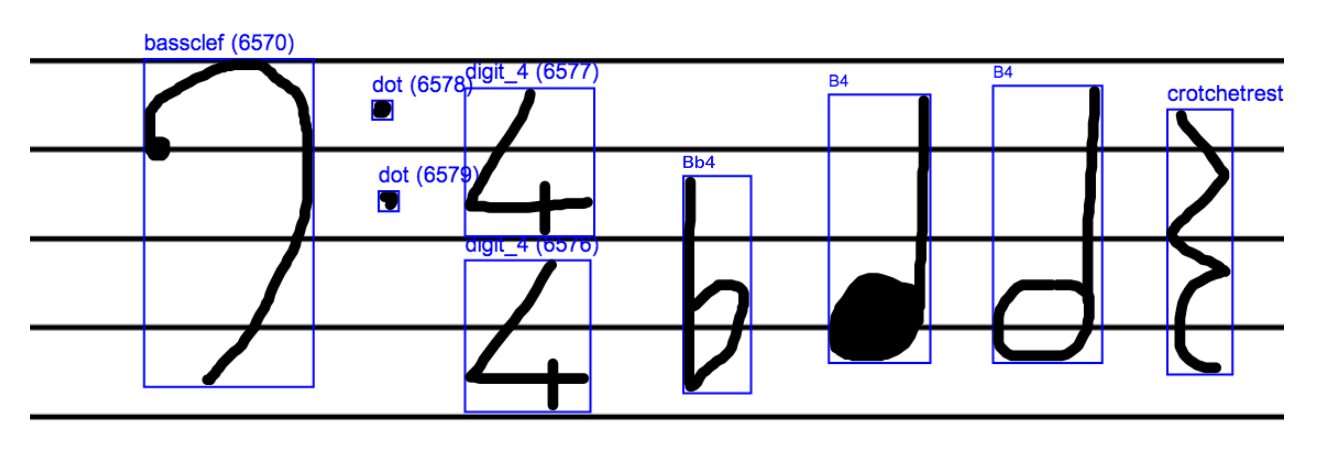
\includegraphics[width=\linewidth]{gfx/techniques/labelling/pitch.png}
  \caption{The manuscript after pitch analysis}
  \label{fig:canvas-pitches}
\end{figure}

For a rough estimate of note head position, the simplest method is to use a known position along the vertical axis, then use that as an estimate for the centre, indeed that's often what is done in standard OMR. However we can get a more accurate position using alternative techniques.

\subsubsection{Sharp Centres}
For the sharp centre, the centroid proved less than satisfactory as it was easily affected by the length of the lines (see the blue centres in \cref{fig:sharp-centroids}), whereas in reality the `centre' of a sharp is determined by the position of its island region in the middle.

By inverting the image and performing connected component segmentation, we can isolate the island region and after extracting the centroids from this region, we get a much more satisfactory identification of the sharp's centre, show in \cref{fig:sharp-centroids} by the intersecting red lines.

\begin{figure}[h!]
    \centering
    \begin{subfigure}[b]{.3\linewidth}
        \centering
        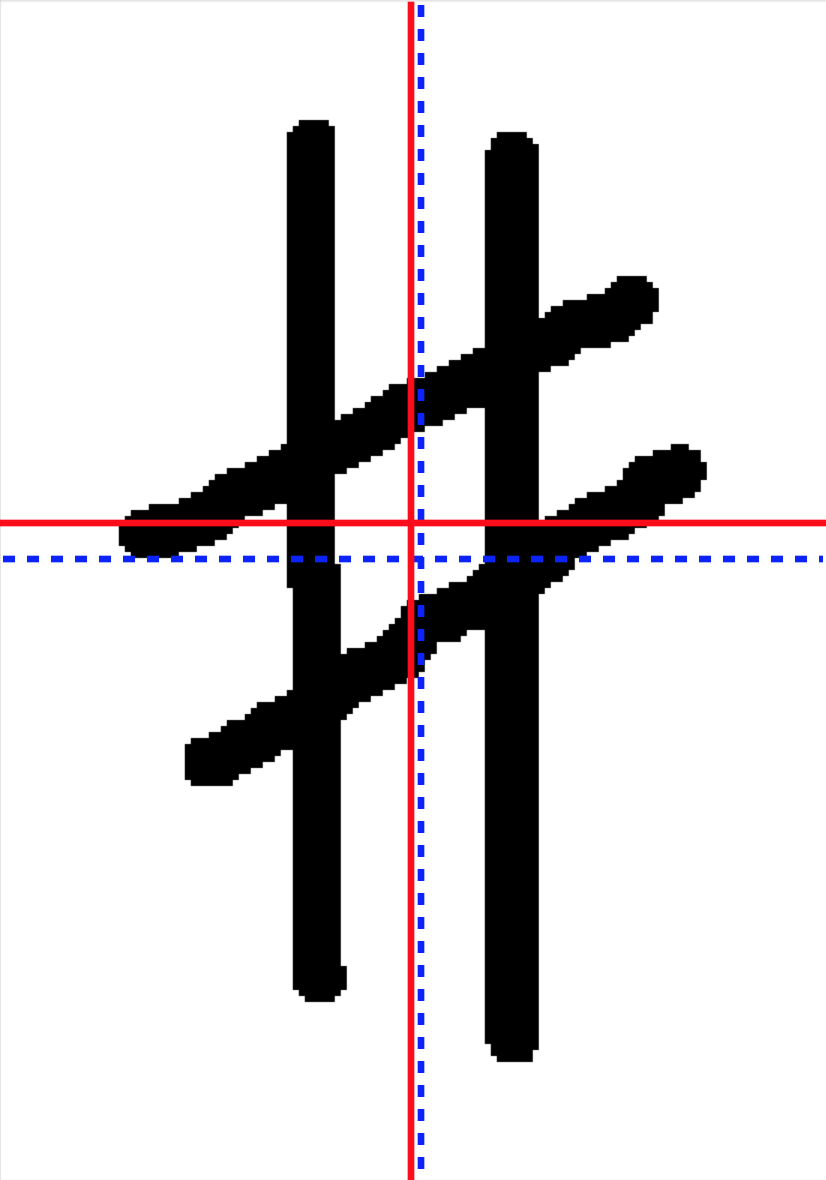
\includegraphics[height=5cm]{gfx/techniques/sharp-centroid-6109.png}
        \phantomsubcaption
    \end{subfigure}
    \begin{subfigure}[b]{.3\linewidth}
        \centering
        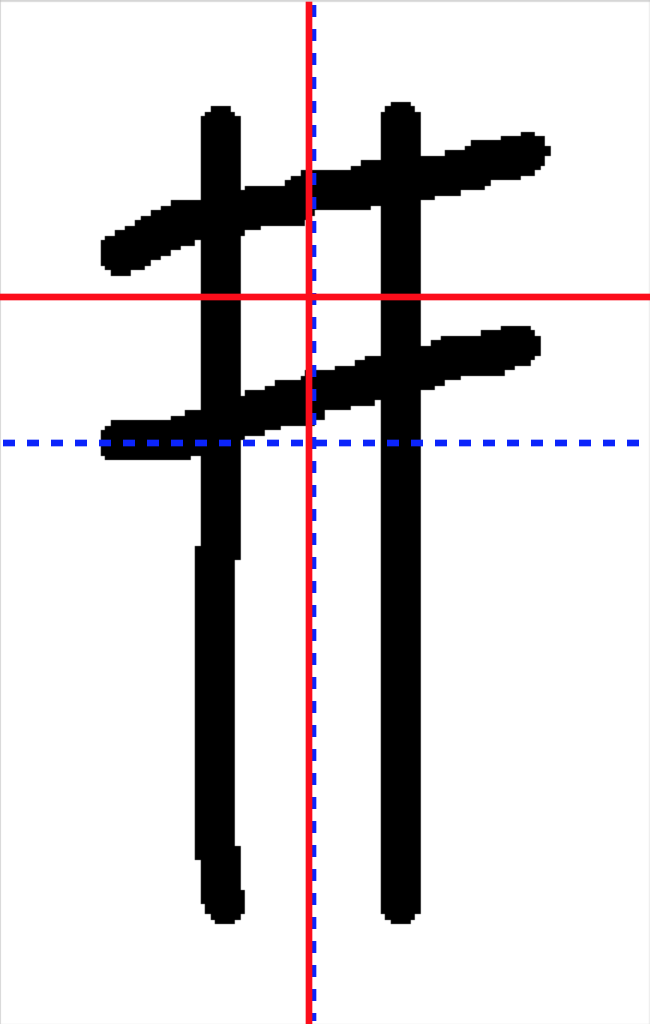
\includegraphics[height=5cm]{gfx/techniques/sharp-centroid-6110.png}
        \phantomsubcaption
    \end{subfigure}
    \begin{subfigure}[b]{.3\linewidth}
        \centering
        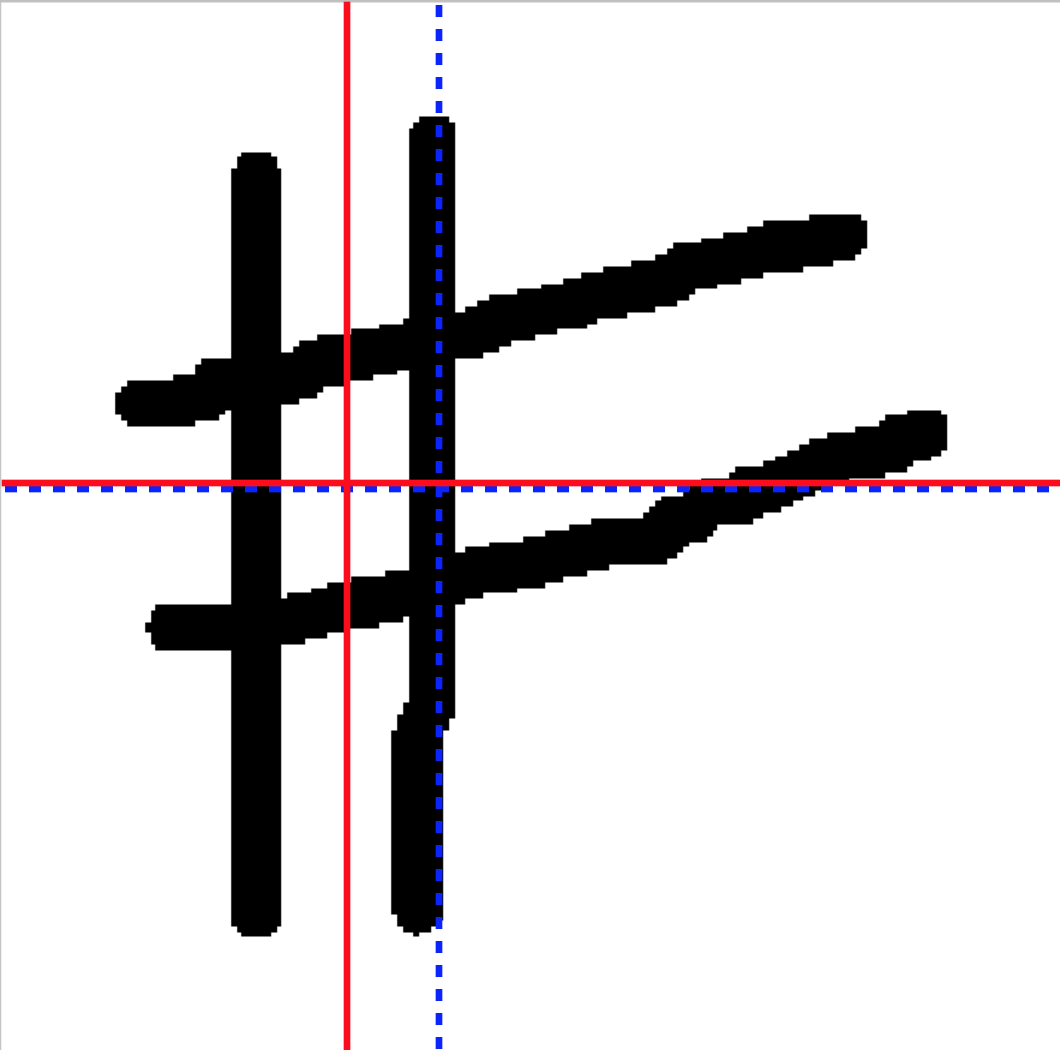
\includegraphics[height=5cm]{gfx/techniques/sharp-centroid-6108.png}
        \phantomsubcaption
    \end{subfigure}

  \caption{Identifying the true centres of the drawn sharps. Red intersecting lines show the true centres and blue intersecting lines show the centroid centres}
  \label{fig:sharp-centroids}
\end{figure}

\subsubsection{Flat Centres}

An unfortunate occurrence in flats during preliminary user testing was that of not joining the head up properly, an example of which can be seen in \cref{fig:flat-broken}. Ideally we would like to perform a similar technique to sharps, however we need some reliable way to compensate for potential breaks.

The first experiment I ran was to perform watershed segmentation by computing a distance transform on the flat, then by using the local maximum peaks as a starting point watershed segmentation was performed, resulting in the initial segmentation seen in \cref{fig:flat-broken-watershed}. From there, by merging neighbouring regions from smallest to largest, we can identify the `island' component (\cref{fig:flat-broken-merged}) and take the y coordinate of the centroid of this region.

\begin{figure}[H]
    \centering
    \begin{subfigure}[b]{.19\linewidth}
        \centering
        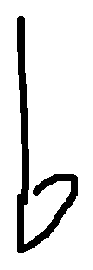
\includegraphics[height=5cm]{gfx/techniques/scoring/flats/6193-original.png}
        \caption{Original}
        \label{fig:flat-broken}
    \end{subfigure}
    \begin{subfigure}[b]{.19\linewidth}
        \centering
        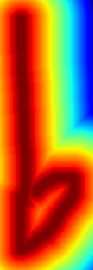
\includegraphics[height=5cm]{gfx/techniques/scoring/flats/6193-distance.png}
        \caption{Distance}
    \end{subfigure}
    \begin{subfigure}[b]{.19\linewidth}
        \centering
        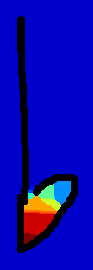
\includegraphics[height=5cm]{gfx/techniques/scoring/flats/6193-watershed.png}
        \caption{Watershed}
        \label{fig:flat-broken-watershed}
    \end{subfigure}
    \begin{subfigure}[b]{.19\linewidth}
        \centering
        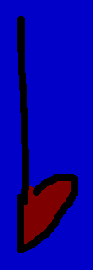
\includegraphics[height=5cm]{gfx/techniques/scoring/flats/6193-segmented.png}
        \caption{Merged}
        \label{fig:flat-broken-merged}
    \end{subfigure}
    \begin{subfigure}[b]{.19\linewidth}
        \centering
        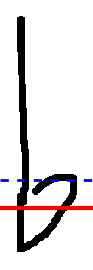
\includegraphics[height=5cm]{gfx/techniques/scoring/flats/6193-center.png}
        \caption{Centre}
    \end{subfigure}

  \caption{Identifying flat centre with watershed segmentation}
  \label{fig:flats-centre-watershed}
\end{figure}

An alternative solution uses dilations. This involves expanding the drawn image (and consequently shrinking the flat's `head' region) evenly until a distinct island region is formed (\cref{fig:flat-dilation}). Once that happens the vertical centre of the `head' can be established in the same way as outlined previously, using the centroid.

\begin{figure}[H]
    \centering
    \begin{subfigure}[b]{.2\linewidth}
        \centering
        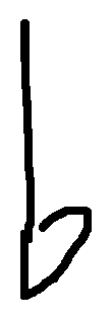
\includegraphics[height=5cm]{gfx/techniques/scoring/flats/6193-dilation-original.png}
        \caption{Original}
    \end{subfigure}
    \begin{subfigure}[b]{.2\linewidth}
        \centering
        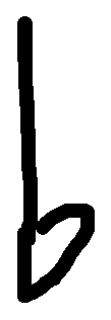
\includegraphics[height=5cm]{gfx/techniques/scoring/flats/6193-dilation-dilated.png}
        \caption{Dilation}
        \label{fig:flat-dilation}
    \end{subfigure}
    \begin{subfigure}[b]{.2\linewidth}
        \centering
        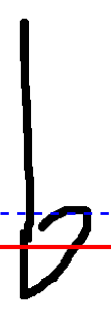
\includegraphics[height=5cm]{gfx/techniques/scoring/flats/6193-dilation-center}
        \caption{Centre}
    \end{subfigure}

  \caption{Identifying flat centre with dilation and connected component segmentation}
  \label{fig:flats-centre-dilation}
\end{figure}

\subsubsection{Note Head Centres}

For note heads, it was discovered that the centroid was a good representation of the centre, even in case of broken minims as seen in \cref{fig:broken-minim}

\begin{figure}[H]
    \centering
    \begin{subfigure}[b]{.32\linewidth}
        \centering
        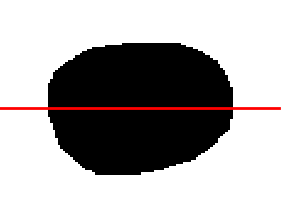
\includegraphics[width=\linewidth]{gfx/techniques/scoring/note-head/1906-centroid-centre.png}
        \caption{Crotchet Head}
    \end{subfigure}
    \begin{subfigure}[b]{.32\linewidth}
        \centering
        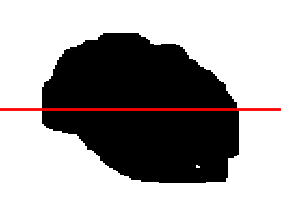
\includegraphics[width=\linewidth]{gfx/techniques/scoring/note-head/6189-centroid-centre.png}
        \caption{Wonky Crotchet Head}
    \end{subfigure}
    \begin{subfigure}[b]{.32\linewidth}
        \centering
        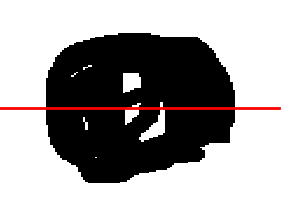
\includegraphics[width=\linewidth]{gfx/techniques/scoring/note-head/6192-centroid-centre.png}
        \caption{Inconsistent Crotchet Head}
    \end{subfigure}

    \begin{subfigure}[b]{.3\linewidth}
        \centering
        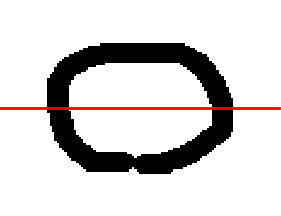
\includegraphics[width=\linewidth]{gfx/techniques/scoring/note-head/1818-centroid-centre.png}
        \caption{Minim Head}
    \end{subfigure}
    \begin{subfigure}[b]{.3\linewidth}
        \centering
        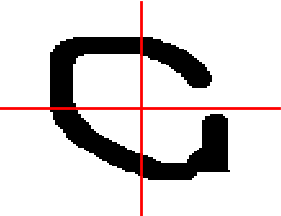
\includegraphics[width=\linewidth]{gfx/techniques/scoring/note-head/6105-centroid-centre.png}
        \caption{Broken Minim Head}
        \label{fig:broken-minim}
    \end{subfigure}

  \caption{Filled and hollow note heads with their centres identified by two red intersecting lines}
  \label{fig:ccl-two-pass}
\end{figure}

\subsection{Duration}
\label{sec:duration-identification}

There are two main steps to the process for calculating note duration. The first is the extraction of the fundamental note value, is it a semibreve, minim, crotchet, quaver or semiquaver? For a  semibreve, the note value will always be four, however for other notes, things are not so straightforward.

We first examine each note individually to ascertain the components which make up the note duration and then assign it a base value. For example we are particularly interested in the note head (is it solid or hollow?) and any tails or beaming. An outline of this heuristic can be seen in \cref{fig:note-duration-flow-chart}.

The number of tails is fairly straightforward as they are attached to isolated notes or are they joined in a more complex beam such as that in \cref{fig:complex-beam-establish}. however, we need to have some way to work out which notes have which values. To do this, a section the width of $\text{Stave Space} / 2$ is examined either side of the note's head. The beam is analysed in these segments for the maximum number of vertical black runs which represents the number beams.

\begin{figure}[H]
  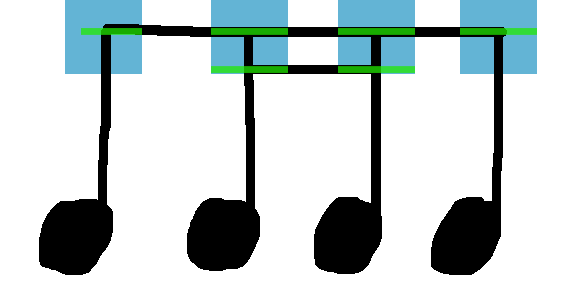
\includegraphics[width=\linewidth]{gfx/implementation/beam-identification.png}
  \caption{Calculating the number of beams to get note values. Blue areas show the regions scanned and green lines represent the maximum count of vertical black runs found}
  \label{fig:complex-beam-establish}
\end{figure}

\begin{figure}[H]
  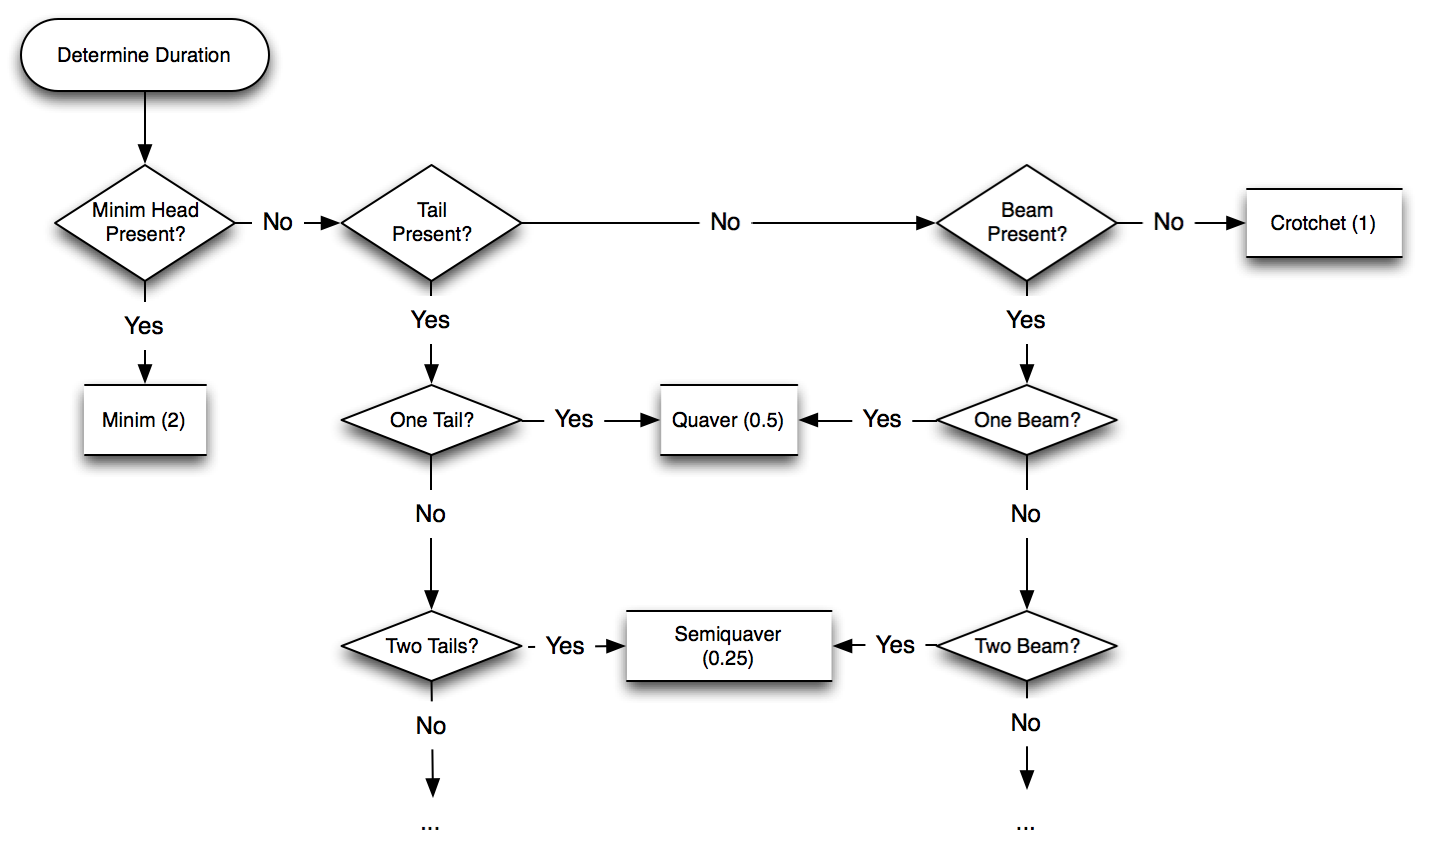
\includegraphics[width=\linewidth]{gfx/implementation/duration-diagram.png}
  \caption{Flow chart for establishing base note duration}
  \label{fig:note-duration-flow-chart}
\end{figure}

Note that with regards to tails and beaming, since every additional beam or tail present for the note divides it's value by two (examples can be seen in \cref{table:note-lengths}) we can generalise this section of the heuristic to deal with any number of beams and tails.

An example of a manuscript where the basic durations have been calculated can be seen in \cref{fig:canvas-durations}

\begin{figure}[hbt]
  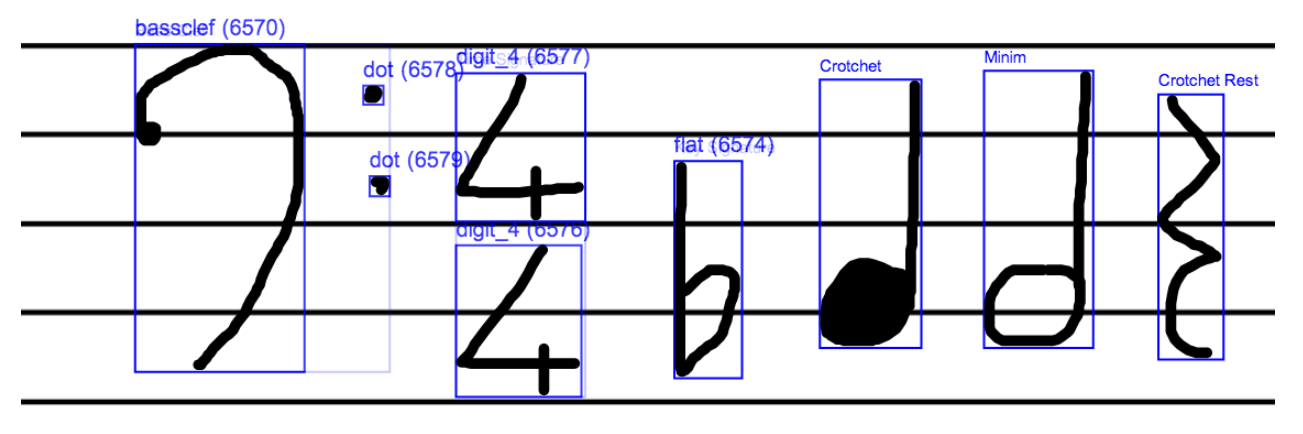
\includegraphics[width=\linewidth]{gfx/techniques/labelling/duration.png}
  \caption{The manuscript after component duration analysis}
  \label{fig:canvas-durations}
\end{figure}

Once the base value has been obtained, we perform a final check of the area surrounding the note centre for any `modifier' dots. These extend the duration of the note by half, so for example, a dotted crotchet would last 1.5 beats as opposed to 1 beat without the dot. The region searched equates to half a staff space down and either side of the note as shown in \cref{fig:identify-dot}, anything outside of this region is ignored.

\begin{figure}[H]
  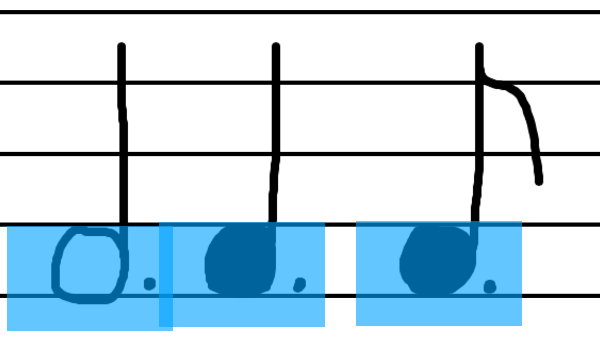
\includegraphics[width=\linewidth]{gfx/implementation/dot-identification.png}
  \caption{Searching for dots which would modify a note's length. Blue areas are the searched space for each note}
  \label{fig:identify-dot}
\end{figure}

\subsection{Domain Knowledge}
\label{sec:identification-domain-knowledge}

After all the segmentation, classification, pitch and duration analysis we can use domain knowledge as outlined in \cref{sec:arebelo-domain-knowledge,sec:domain-knowledge-taubman} to apply musical rules (with looser thresholds and variations in control flow to account for the potential mistakes like those in \cref{sec:common-manuscript-mistakes}) to group components as seen in \cref{fig:canvas-domain-knowledge}, enabling scoring \cref{sec:scoring} of the manuscript.

\begin{figure}[hbt]
  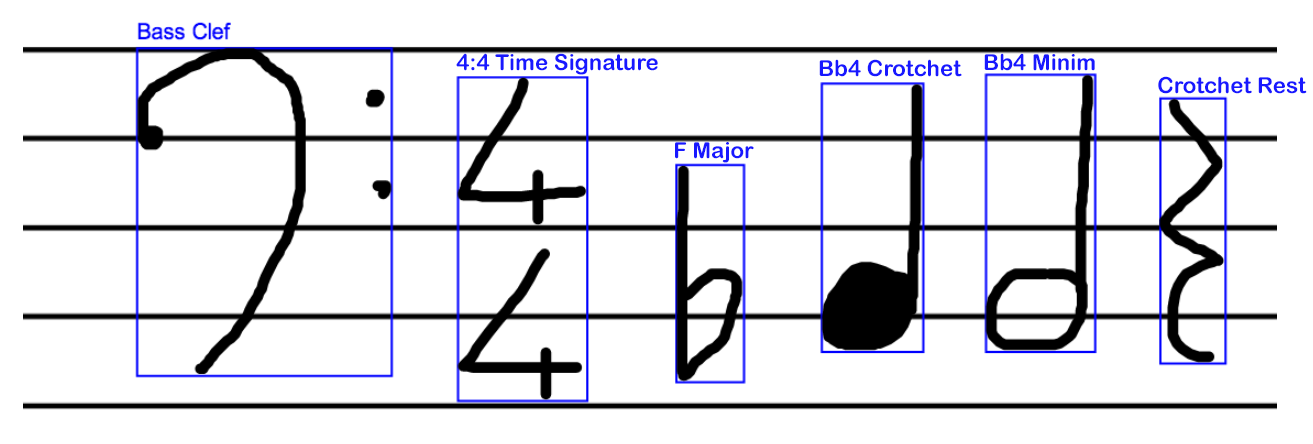
\includegraphics[width=\linewidth]{gfx/techniques/labelling/domain-knowledge.png}
  \caption{The manuscript after application of domain knowledge. Note the time signature, key signature and clef components have been grouped correctly}
  \label{fig:canvas-domain-knowledge}
\end{figure}
